\chapter{Similarity Analysis}

\section{Parse Tree Kernel Algorithm for Projects}

To perform the actual similarity measure between two files, we use the 
parse tree kernel function as defined in the background section (\cpageref{sec:parseTreeKernel}).
After breaking up the projects into individual files, 
the algorithm iterates over every file from the first project, comparing
the parse tree of each with the tree of every file in the second project. 

The similarity function iterates over every node in the first tree, and
for each node in the second tree, adds the result of the node comparison to
a running total. To compare the nodes, we ignore a lot of the specifics of
the node, and only consider ASTNodes of the same subclass to be equal.

We ignore information such as variable name or name of method invoked as
across submissions, these values will frequently vary, whilst the semantics
of the program remain the same. For example consider the code snippets from
\cpageref{Background} reproduced here, \cref{fig:xyzForLoop} and \cref{fig:ijkForLoop}
The two loops perform the exact same function, and none of the variables share
the name.

If the types of node don't match, as is the case for most node comparisons,
we immediately return 0. Otherwise, we set the value of this similarity to be
the same as the \emph{decay factor} heuristic, then iterate over the sets of children of the
compared nodes. For each child, we multiply the similarity of the parent node
by 1 + (the maximum similarity of this child with the other node's children).
This maximum is calculated recursively, with maximum recursive depth being
the same as the \emph{threshold depth} heuristic, or terminating once a leaf
node has been reached, whichever is earlier.

To actually perform 
the comparison, we utilise a number of classes, both to set up the tree, then to actually
compare the two. First, we use the in built Java parser -- \texttt{org.eclipse.jdt.core.dom.ASTParser}
-- to generate an \texttt{ASTNode}. Unfortunately, the default eclipse ASTNode is difficult
to navigate; though it takes the form of a tree structure, depending on the ASTNode 
type (e.g. Class Definition vs Unary Operator), different methods are used to traverse
the tree and this results in the traversal being non-trivial. To counter this, we
used a visitor pattern to visit every node in the tree. Our class, \texttt{AllNodeVisitor},
is accepted by the \texttt{ASTNode}, as it extends \texttt{ASTNodeVisitor}. Once accepted, it visits
every node in the tree, first visiting the root node, then all of it's children in 
order. When the \texttt{AllNodeVisitor} visits a node, the 
\texttt{preVisit(ASTNode node)} method is called, and here we
create an \texttt{ASTNodeWithChildren}, passing in the current \texttt{ASTNode} as the node. The 
\texttt{ASTNodeWithChildren} is used later as a convenience class to easily traverse
the tree, countering the problem described above. A \texttt{Stack} keeps track
of the parents of each node, and the children are added when they're visited.
Once the whole parse tree has been visited, the \texttt{AllNodeVisitor} has an 
\texttt{ASTNodeWithChildren} holding the root of the AST, and this is passed to
our similarity function.
To perform the comparison of nodes, we get the type of the \texttt{ASTNode} held
in the \texttt{ASTNodeWithChildren}, and match on that.

Further modifications and criticisms of the algorithm are discussed in \cref{Evaluation}.

\begin{figure}
\begin{minipage}[b]{0.45\linewidth}
\begin{lstlisting}
int len = 5;
int[][][] myArr = new int[len][len][len];
for(int x = 0; x < len; x++) {
	for(int y = 0; y < len; y++) {
		for(int z = 0; z < len; z++) {
			myArr[x][y][z] = x+y+z;
		}
	}
}
\end{lstlisting}
\caption{a simple for-loop}
\label{fig:xyzForLoop}
\end{minipage}
\hspace{0.5cm}
\begin{minipage}[b]{0.45\linewidth}
\begin{lstlisting}
int size = 5;
int[][][] nums = new int[size][size][size];
for(int i = 0; i < size; i++) {
	for(int j = 0; j < size; j++) {
		for(int k = 0; k < size; k++) {
			nums[i][j][k] = i+j+k;
		}
	}
}
\end{lstlisting}
\caption{a semantically identical for-loop to \ref{fig:xyzForLoop}}
\label{fig:ijkForLoop}
\end{minipage}
\end{figure}

\section{Individual File Comparison}
\label{sec:SimilarityAnalysis}
In \cref{sec:Two File Comparison View}, we will examine a feature 
our plugin in which we can compare two files (rather than projects) and highlight
the areas of highest similarity. To get a similarity measure between two files
the parse tree algorithm, which is aimed at getting the similarity of a whole
file, needs to be altered so the subtrees of the file can each be compared in a 
normalised manner. The original algorithm iterates over every subtree, calculating
a score for each, but this value is unnormalised until combined with all scores.
As is the case in the main section of the algorithm -- an unnormalised value
will unfairly weight larger trees that perhaps match less well than the
smaller trees.

\chapter{Plugin Design}

\section{Preparation of Source Code}

The students' code is currently stored as a directory of folders, one folder for
each student. Within each student folder, we find the bare git repositories of 
each exercise. Given that the tool is specifically aimed at aiding the lab helpers,
we wanted to automate a way to get this code into eclipse to be used by our plugin.
If the initial work to import the code to Eclipse was too long winded and tedious,
our tool would probably add more time to the analysis of the code, and divert markers'
attention away from actually marking the code.

To achieve this a simple bash script was developed. The script requires git and
maven to be installed on the running machine. The script should be run from the
top directory, with the name of the repository to clone passed in as an argument.
A small amount of modification is needed here depending on the structure of the
source code. Assuming the code is located in the default Java package, a folder
named ``[repository name]\_[username]'' will be created in each student's directory.
Into here we copy a ``generic pom'' file to be used by Maven. The command line tool
sed modifies this file to substitute a unique project name (of the same format as
the new subdirectory name) and then Maven builds the project with the command 
\texttt{mvn compile eclipse:eclipse}. This will compile the program, then generate
Eclipse project files. From here, we can now open up Eclipse and use the 
\texttt{File->Import->Existing Projects into Workspace} and select the top-level
directory as the root directory, allowing us to easily import all projects.

A clean script is also provided to quickly remove any files and folders created with
the previous script.

\section{Project Comparison}

Using the plugin extension points,
we create an entry point to our analyser from our own menu item in Eclipse. This
handler passes an array of the projects in the workspace to our similarity analyser.
The analyser has been structured in a modular manner, allowing future extensions
to be created easily. We have a SimilarityAnalyser abstract class, which takes
care of the setting up of the analyser and holds a number of protected variables
to be used by any implementing classes. For example, the scores are held as a
\texttt{double[][] scores} and this is initialised in the SimilarityAnalyser
constructor such that each dimension is set to be the length of the number of
inputted projects. An ordered list keeps track of which user the scores correspond
to. In setting up the analyser, we check for a skeleton project in the directory,
named [project\_name]\_skeleton\_. If this Directory is found, we create a Set,
which will hold the names of unmodified (and therefore uninteresting) code.

Initially the Parse Tree Analyser was set up to iterate over the projects, and
compare each in turn as defined in the equations discussed in the background 
\cref{eq:parseTreeKernelBase1}, \cref{eq:parseTreeKernelBase2},
\cref{eq:parseTreeKernelRecurse}. Here our implementation makes an assumption about
the algorithm; the algorithm indicates how to get a similarity score between two 
parse trees, however it does not indicate how to perform this measure across a code
base of multiple files. Our implementation finds the maximum similarity of one file
compared with each file from the other project in turn, and uses this value as the
similarity score for that particular parse tree (which is then summed with the similarity
score from each other parse tree). We chose the maximum rather than the mean, as
you might expect with similarity, as the mean method would negatively weight our
similarity even when an exect match is found. For example, if we have a project A
containing 2 files, \texttt{A1.java} and \texttt{A2.java} (which are very different
to each other) and a similar project B with files \texttt{A1.java} and \texttt{B2.java}.
Even if the files in project A are exactly the same as the corresponding files in
project B, using the mean similarity would give us a value of below a perfect match,
which is undesirable in this context.

Once we have a similarity between every project in our workspace, we need a place
to see our results; this is where 
\texttt{com.imperial.fiksen.codesimilarity.utils.ResultsPrinter} comes in.
The SimilarityAnalyser has a print function, which
passes in an OutputStream (usually a stream to the file we want to create) and
there are a number of functions depending on our desired output format; currently
hardcoded to be our Orange output. Once the scores have been outputted, the SimilarityAnalyser
then launches a process of Orange using a generic project setup. This opens a pre-
configured Orange window, holding the distance matrix (i.e. the distance between
each project, or the inverse of their similarities), in a clustered format.

The choices for \emph{threshold depth} and \emph{decay factor} were set at 3 and 0.2
respectively, as discussed in \cref{Evaluation}

\section{Two File Comparison View}
\label{sec:Two File Comparison View}

In viewing the distance map and cluster output, we can see pairs of projects that are
interesting -- for example, looking at the heatmap display,
we could identify an interesting cluster which
appears dissimilar to most of the other submitted code, but very similar to
each other. If we cross reference this with the grades received and see
onsistent grading of these unique outliers, it would be interesting to open
the files together and perform some comparison to see why they are especially
similar. It would be simple to open the files together and perform a manual
inspection, but we were interested in seeing if our similarity algorithm could
be applied on a finer grained level between two files, and highlight areas
of interest.

We developed a proof of concept implementation of this idea inside our plugin.
The view we were looking for would look much like the diff comparison view,
as seen in \cref{fig:diffView}, however the highlighted areas would
be of structurally similar code, and not necessarily in sequential order. Here,
rather than performing the standard diff of text and highlighting the areas
changed, the most similar segments between the two files are identified and
linked together. The match would be defined by some threshold similarity, relative
to the general similarity of the projects.

\begin{figure}[H]
	\centering
		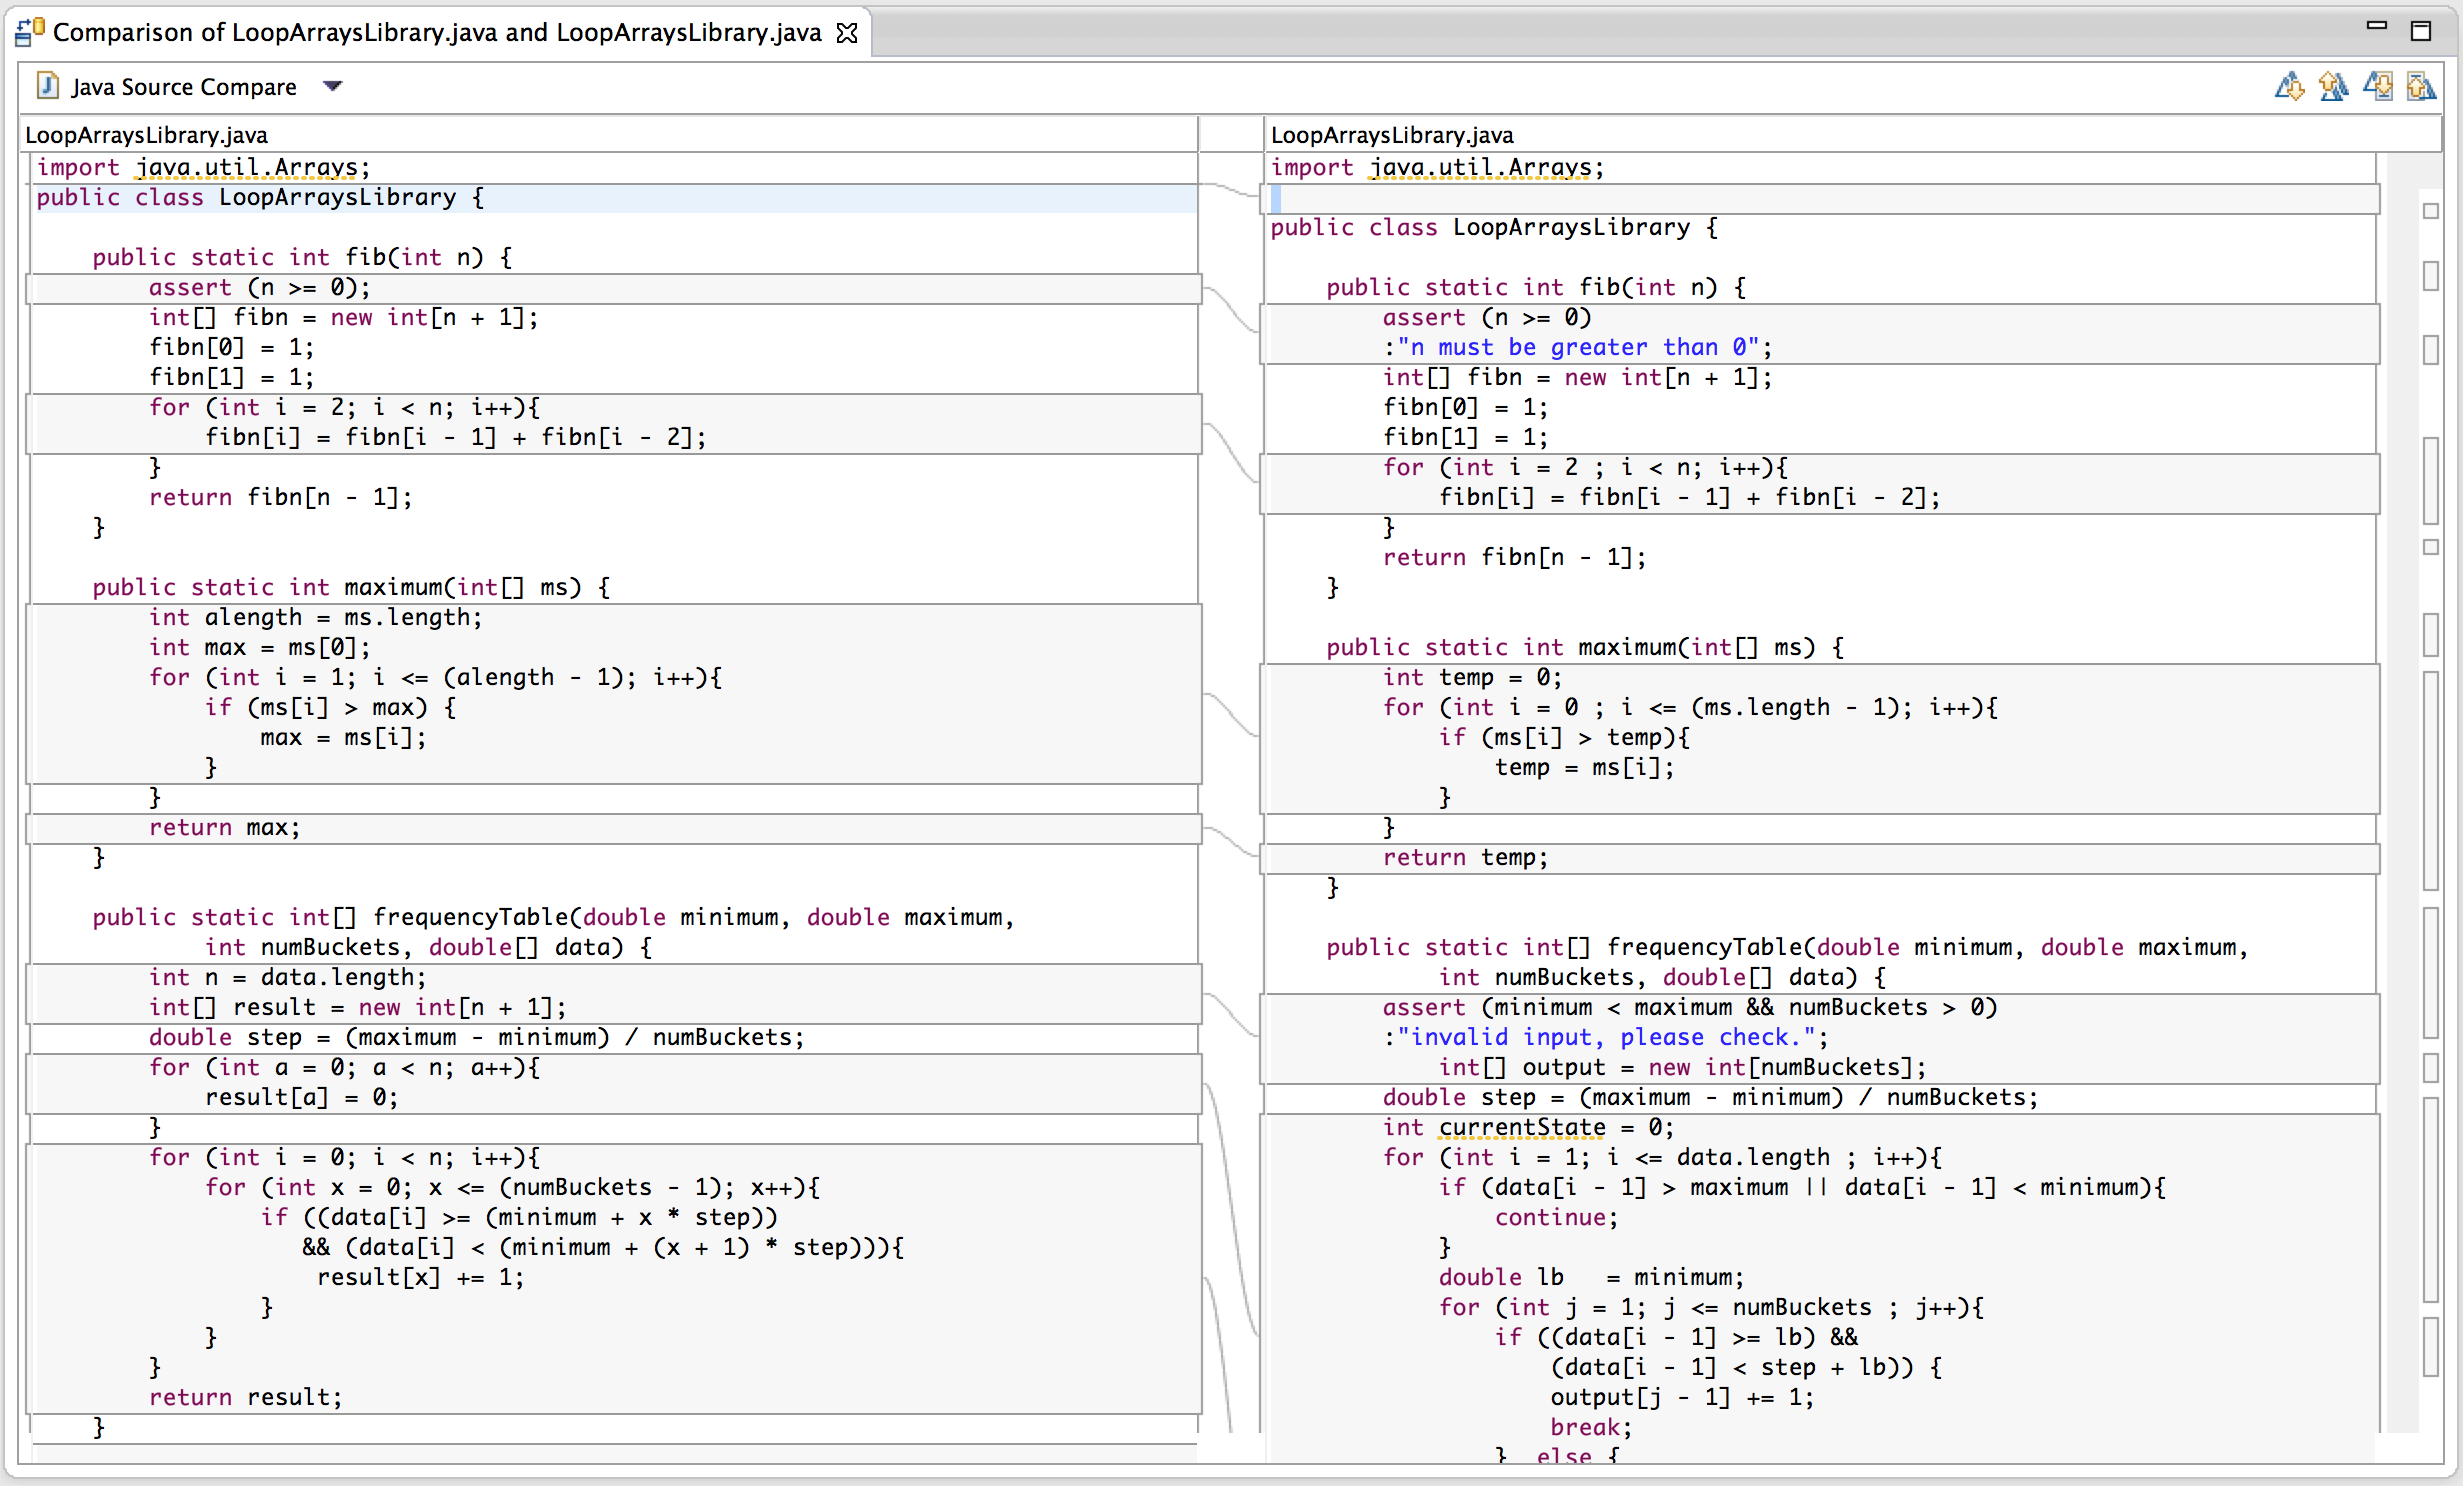
\includegraphics[width=\textwidth]{Figures/EclipseDiffView}
	\caption{The proposed comparison view would closely resemble the current eclipse
	diff view, with a few minor changes}
	\label{fig:diffView}
\end{figure}

To implement this we worked through the eclispe source code, specifically
the org.eclipse.compare packages\footnote{http://goo.gl/hhjWK7}. The documentation
on modifying the differencing engine was sparse and large, complex library 
classes required an ad hoc approach to creating our required classes.
Initially we created another extension in the menu as an entry to our program
and hooked up a new handler to deal with the comparison. This handler opens
up a 2 way comparison between every seleted file, using our custom 
SimilarityCompareEditorInput. The SimilarityCompareEditorInput borrows 
a large amount of code from the eGit
codebase\footnote{https://git.eclipse.org/c/egit/egit.git/tree/}, and is essentially a thinned out version of their
class, providing only primarily skeleton methods that allow us to setup the
configuration of files. 

The custom diff view is then created with dependency injection. Using the
JavaContentViewerCreator\footnote{http://rubenlaguna.com/wp/2007/08/18/eclipse-cvs-compare/}, and extending the extension point
\texttt{org.eclipse.compare.contentMergeViewers}, we generate our ParseTreeMergeViewer.
This class is a copy of the \texttt{TextMergeViewer} Eclipse class, modified to use
its own fields and methods, rather than the inaccessible package protected versions
of the ContentMergeViewer, which is being extended. The primary modification
to this class was the use of ParseTreeDocumentMerger as a replacement for the
original DocumentMerger fMerger object. The ParseTreeDocumentMerger again takes
much of its code from the DocumentMerger built in to Eclipse. A key modification
is present in the doDiff() method, which creates a ParseTreeSimilarityAnalyser,
and runs the compare function on the two documents held by the merger (as 
previously described, this set in the SimilarityCompareEditorInput to be
two of the selected files). The ParseTreeSimilarityAnalyser has additional
methods to create this special comparison for both files, described in 
\cpageref{sec:SimilarityAnalysis}, returning an array of subclass of RangeDifference.
This returned value uses a hack of RangeDifference, which indicates the similar
sections are actually a diff change, and the unsimilar sections are marked
as nochange. This decision was made so we can use the painting methods of the
class with minimal modification.

As this section is somewhat experimental, and with the lack of Eclipse
support for implementing a plugin of this type, the end result was a scaled
back version of our initial vision. In \cref{fig:finalCodeCompare} we see
our result. We can see the green bar on the right indicating the most similar
methods of the two classes; selecting this green bar highlights the similar
methods in both source files.

\begin{figure}[H]
	\centering
		\includegraphics[width=\textwidth]{Figures/FinalCodeCompare}
	\caption{The final, scaled back version of individual file comparison}
	\label{fig:finalCodeCompare}
\end{figure}


\chapter{Implementation Improvements}

\section{Algorithm}

A number of issues arose with the algorithm, requiring modifications to fit our
needs. 

\subsection{Multiple Classes and Packages}

The parse tree kernel algorithm is also limited in its ability to compare only
single files with each other, so we must provide our own implementation for
an extension to deal with many files per project. Our extension simply continued
the the algorithm's pattern -- the files were compared with each other, and for
each file in the first list, the maximum similarities with files in the second
list are multiplied together, with the threshold value. In doing this, we essentially
treat each file as the root node of the tree.

\subsection{Removal of Uninteresting Code}

As the submission system in which students hand in code is automated, the 
skeleton repository is automatically submitted for students who fail to attempt
the coursework. If we retain the results of these users, we end up with a
distance heatmap as seen in \cref{fig:skeletonHeatmap} (for more information on
the heatmap results, see \cref{Evaluation}). The bright yellow/orange section indicates
a large distance from the submission. In retaining these results, we only serve to
hide information in the heatmap -- the unmodified submissions all cluster perfectly
with each other and poorly with the other data sets, they actually tell us no added
information about the results, thus we delete these results.

\begin{figure}[H]
	\centering
		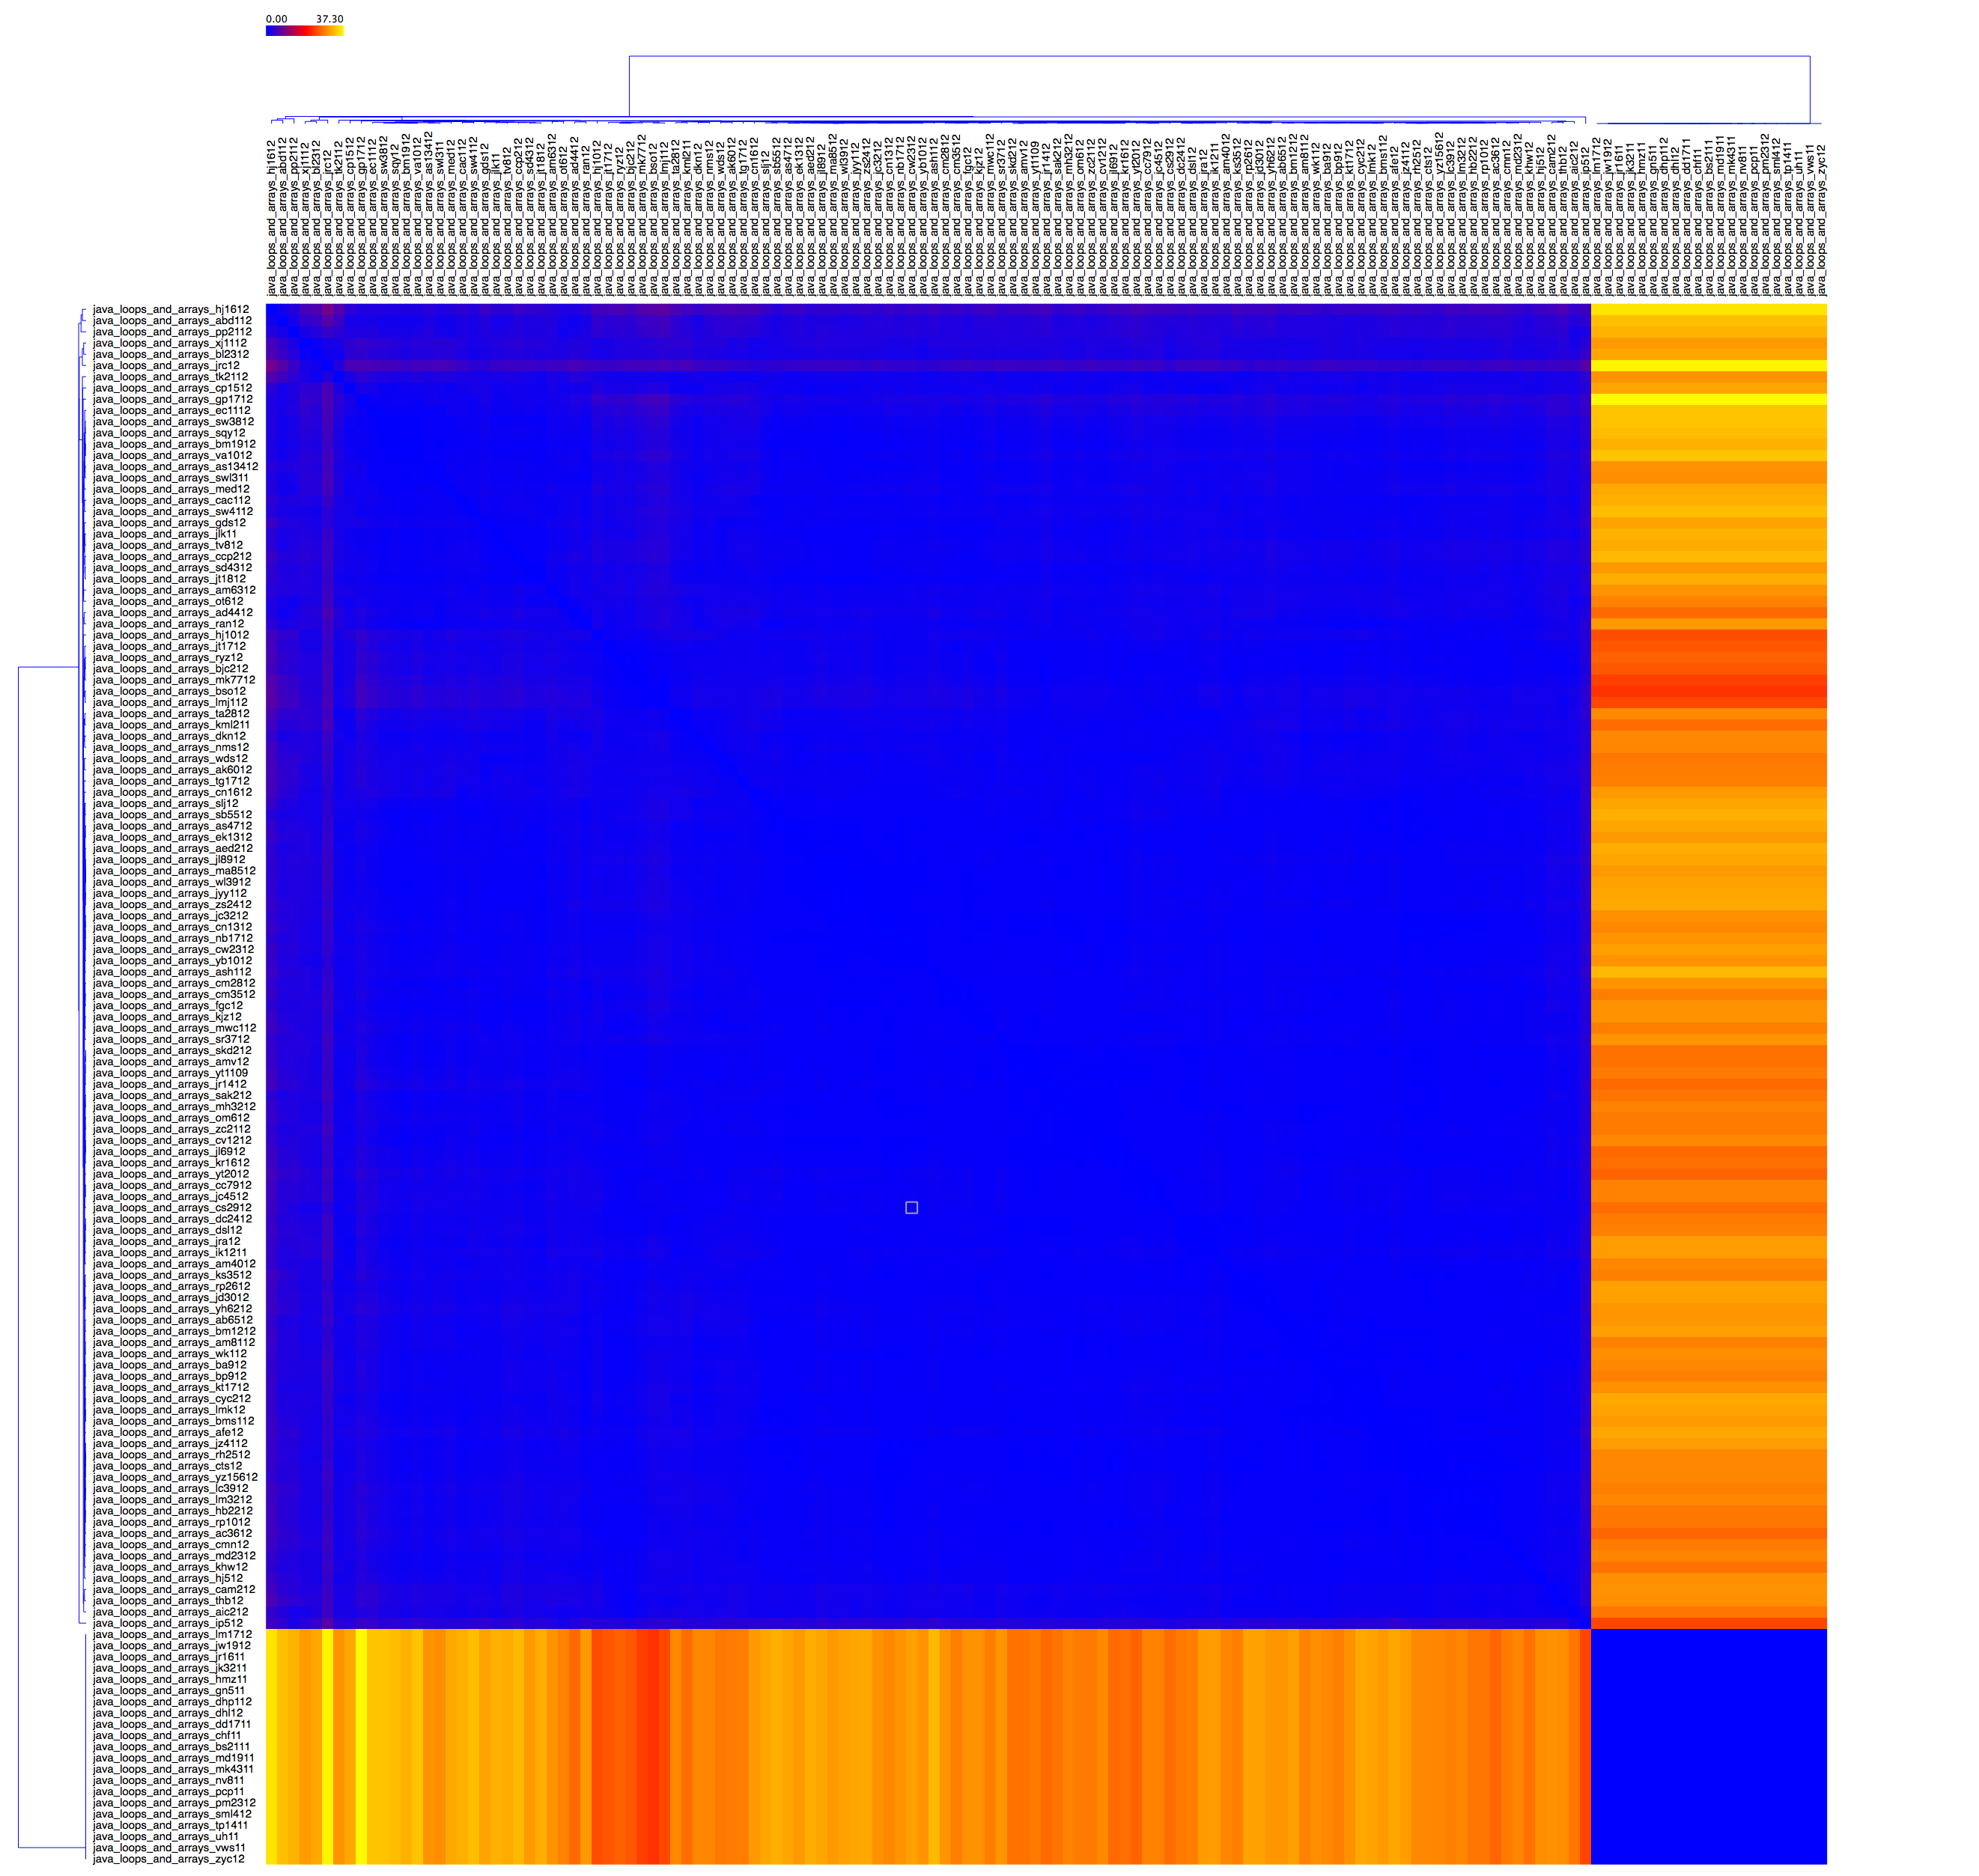
\includegraphics[width=\textwidth]{Figures/LoopArraySkeletonHeatmap}
	\caption{Results heatmap with unmodified code results left in}
	\label{fig:skeletonHeatmap}
\end{figure}

\section{Threading}

The structure of the program was modified from a single threaded implementation to
increase program performance.

There are multiple places threading is used to better the algorithms 
implementation. The handler initially sets off the analysis in its own thread
this frees up the main UI thread so the user isn't frozen out of
Eclipse until the analysis completes.

When performing the actual comparisons, we make heavy use of threading and caching
to parallelise computation. 2 threads per processor are set off, computing the similarity
of files. Each thread takes on $\frac{1}{num threads}$ projects, 
comparing their projects against the whole set. The current implementation relies on the
assumption that all projects are roughly the same size, and so an intelligent
assignment of tasks is unneeded -- each thread takes the project's whose positions
satisfy $pos \% num threads == thread ID$. The speed up is reasonable, with
a full data set comparison of projects reducing from 86 to around 42 seconds on
a quad core processor with hyperthreading (i.e. 8 threads).

